\section{Introduction}
\label{sec:intro}

Adversarial training remains the most reliable defense against norm-bounded attacks
\citep{PGD,athalye2018obfuscated,AutoAttack}, but its robustness comes with lower accuracy on clean
inputs. This trade-off is partly intrinsic to the training objective \citep{tsipras2018robustness,TRADES}
and becomes especially restrictive for compact networks. Existing approaches improve the target seen
during adversarial training: some replace one-hot labels with softened or self-distilled targets
\citep{pang2020bag,tack2022consistency,adr}, while adversarial distillation transfers predictions from
a robust teacher \citep{ard,iad,rslad,adaad,igdm}. The latter can be effective, but presupposes a model
that has already paid the cost of robust training.

A naturally trained copy of the student has the complementary property: it is inexpensive and holds
the clean accuracy that adversarial training loses, but it is itself non-robust. Prior methods use such
a model as auxiliary guidance. ARREST preserves its representations alongside a label objective
\citep{arrest}; DP-FAT rescales its logits per example \citep{dpfat}; and B-MTARD balances it against a
second, robust teacher \citep{bmtard}. These designs raise a more basic question: \emph{can a natural
teacher provide the sole supervision for adversarial training, without transferring its fragility?}

\begin{figure}[t]
  \centering
  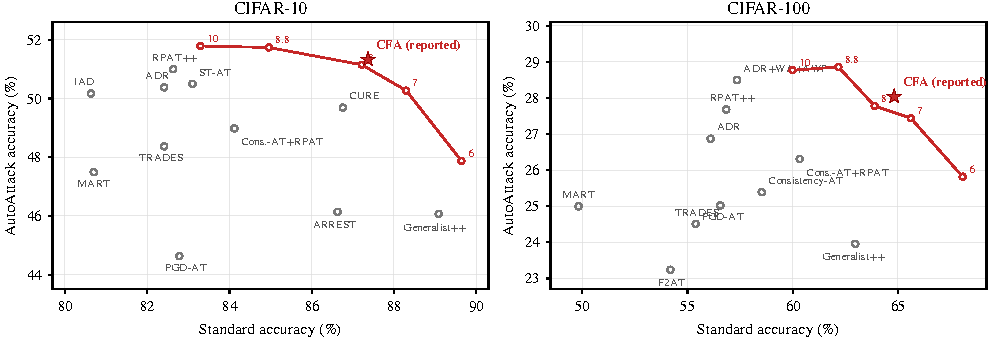
\includegraphics[width=\linewidth]{figure/frontier.pdf}
  \caption{Clean--AutoAttack trade-off on CIFAR-10 and CIFAR-100 with ResNet-18 at
  $\epsilon=8/255$. Grey points
  are published results (\Cref{tab:published}); the CFA curve varies the training radius, and the star
  marks the configuration used elsewhere.}
  \label{fig:frontier}
\end{figure}

Our approach separates the teacher's role as a clean target from the student's response to
perturbations. The teacher supplies a representation at the clean input; the student learns to
preserve it throughout the perturbation set, without matching the teacher at perturbed inputs.
We instantiate this principle as \textbf{Clean Feature Anchoring} (CFA): adversarial training uses
feature regression as the entire backbone objective and retains the teacher's classifier.
Softening probability targets improves robustness in our experiments, but direct regression offers
a competitive alternative without temperature selection. Logit regression is also effective;
the central finding is that clean-target regression can replace, rather than supplement, label supervision.

This single target has a useful structural property. Let $L$ denote the worst-case distance from the
student feature to the clean teacher feature, $F$ the clean teacher--student discrepancy, and $O$ the
diameter of the student's features over the perturbation ball. We show that
$L\le F+O\le3L$. Thus the same objective controls teacher fidelity and local variation without
balancing separate penalties. The result does not certify robust classification, but it explains why
removing the label loss does not leave stability unconstrained.

We further address a mismatch left by a uniform attack radius. The radius is measured in pixels,
whereas CFA measures displacement in feature space, so equal pixel budgets can induce very different
loss changes across examples. Our sensitivity-matched radius assigns less budget to locally sensitive
examples and more to insensitive ones while preserving the batch total. This allocation improves both
axes over the uniform-radius anchor and introduces no additional loss term.

CFA achieves competitive clean--robust trade-offs across CIFAR-10, CIFAR-100, and
Tiny-ImageNet. On CIFAR-100 with ResNet-18 it reaches $62.17\%$ clean and $28.86\%$ AutoAttack
accuracy (\Cref{fig:frontier}). Controlled experiments show that the gain persists without weight
averaging or adversarial weight perturbation, and that substituting label cross-entropy under matched
training conditions reduces both clean and robust accuracy. Varying the natural-teacher checkpoint
reveals that increasing teacher clean accuracy can reduce student clean accuracy while improving
robustness. Changes in the teacher's class separation are also reflected in the student, suggesting
that teacher selection should consider the resulting student trade-off.

Our contributions are threefold:
\begin{itemize}
  \item We show empirically that a natural teacher can supply the sole target for adversarial
  training. CFA realizes this with clean feature regression and an inherited classifier, without
  a label loss or temperature selection during robust training.
  \item We characterize how a fixed anchor controls fidelity and local feature variation, and develop
  a sensitivity-based radius allocation whose benefit persists when the radius distribution is controlled.
  \item Across three datasets and two architectures, we evaluate transfer beyond label training and
  recipe effects, and show that higher teacher clean accuracy need not improve student clean accuracy.
\end{itemize}
